\documentclass{IEEEtaes}

\usepackage{color,array,amsthm}
\usepackage{graphicx}
\usepackage{amsmath}
\usepackage{algorithm}
\usepackage{algpseudocode}
\usepackage{soul}
\usepackage{subcaption}
\renewcommand{\algorithmicrequire}{\textbf{Input:}}
\renewcommand{\algorithmicensure}{\textbf{Output:}}
\newcommand{\algrule}[1][.1pt]{\par\vskip.2\baselineskip\hrule height #1\par\vskip.5\baselineskip}


\usepackage[outline]{contour}% http://ctan.org/pkg/contour
\usepackage[letterspace=50]{microtype}
\contourlength{0.2pt}
\contournumber{10}%

\jvol{02}
\jnum{2307668}
\jmonth{Fall}
\paper{1234567}
\pubyear{2023-24}
\doiinfo{TAES.2020.Doi Number}

\newtheorem{theorem}{Theorem}
\newtheorem{lemma}{Lemma}
\setcounter{page}{1}
%% \setcounter{secnumdepth}{0}



\begin{document}

\title{\contour{black}{\textbf{An Approach}}
       \contour{black}{\textbf{to n-Dimensional}} \\
       \contour{black}{\textbf{Path Planning}} \\
       with \\ Potential Functions \\
       }


\author{OZGUR GULSUNA}
\member{2307668}
\affil{Middle East Technical University, Ankara, TR} 

%% \author{FOURTH D. AUTHOR}
%% \affil{University of Colorado, Colorado, USA}

\receiveddate{Manuscript received XXXXX 00, 0000; revised XXXXX 00, 0000; accepted XXXXX 00, 0000.\\
%% This paragraph of the first footnote will contain the date on which you submitted your paper for review, which is populated by IEEE. It is IEEE style to display support information, including sponsor and financial support acknowledgment, here and not in an acknowledgment section at the end of the article. For example, ``This work was supported in part by the U.S. Department of Commerce under Grant BS123456.'' }
%% \accepteddate{XXXXX XX XXXX}
%% \publisheddate{XXXXX XX XXXX}

% \corresp{The name of the corresponding author appears after the financial information, e.g. {\itshape (Corresponding author: M. Smith)}. Here you may also indicate if authors contributed equally or if there are co-first authors.}

% \authoraddress{The next few paragraphs should contain the authors' current affiliations, including current address and e-mail. For example, First A. Author is with the National Institute of Standards and Technology, Boulder, CO 80305 USA 
% (e-mail: \href{mailto:author@nrim.go.jp}{author@nrim.go.jp}).}

\editor{}
\supplementary{}


% \markboth{AUTHOR ET AL.}{SHORT ARTICLE TITLE}
\maketitle

\begin{abstract}\textls{This} study explores the intricacies of robot motion planning in higher dimensions, deliberately excluding dimensions below two for depth. Detailing the robot's interaction with an n-dimensional environment and complex obstacles, the proposed Potential Function Approach employs conic and quadratic functions for attraction and dynamic adjustments for repulsion. Solver selection integrates ODE45 for accuracy and a discrete iterative solver for flexibility. Implementation intricacies, including obstacle representation through bounding n-spheres, address computational trade-offs. Experimentation ranges from 2D scenarios to 3D, seeking insights into effective motion planning within a MATLAB simulation environment. The study offers a concise exploration of path planning challenges in multi-dimensional spaces.
\end{abstract}


\begin{IEEEkeywords}Motion Planning, Potential Functions, High Dimensions, Hypersphere, MATLAB, Simulation.
\end{IEEEkeywords}
\vfill\null




\section{\large \textbf{Introduction}}


{\scshape T}his exploration delves into the challenges of robot motion planning in higher dimensions, deliberately focusing on dimensions greater than two for a nuanced investigation. It details the robot as a single-point entity within an n-dimensional environment, navigating static obstacles of varying complexities. The deliberate absence of repulsive systems from soft borders adds complexity to the robot's interaction with its environment, progressing from simple points to intricate high-dimensional geometric configurations.

The utilized approach introduces additive attractive and repulsive potentials, with conic and quadratic functions for attraction and repulsion based on obstacle proximity. Employing Gradient Descent for goal-reaching, the implementation integrates both ODE45 for accuracy and a discrete iterative solver for flexibility in solver selection, unraveling advantages and trade-offs across dimensions.

Implementation include obstacle representation through bounding n-spheres, accuracy trade-offs between exact and approximate representations. Experimentation spans 2D scenarios to eliminate local minima challenges and extends to 3D, visually representing potential functions in complex environments. The study seeks insights into effective robot motion planning in intricate spaces, offering a comprehensive exploration within a MATLAB simulation environment, aiming to deepen understanding of path planning challenges in multi-dimensional spaces.
% n-dim meaning that have a dim number that is arbitrary, positive and integer
\section{\large \textbf{Problem Definition}}

\begin{figure}[t!]
    \centering
    \vspace{0.5em}
\end{figure}

The implementation begins with a precise definition of the robot, environment, and obstacles. These definitions are constructed to allow for mathematical concepts to be generalized seamlessly to higher spatial dimensions, requiring little to no modification in observations and interactions with the environment.

This work specifically engages with dimensions higher than two. This choice is deliberate, as navigating one-dimensional environments and obstacles presents a balance of being straightforward and complex simultaneously. Moreover, the notion of an "obstacle" itself poses a challenge to finding a "suitable path" solution in a single dimension. However, there exist a distinct research-area in the domain of list-type path planning tasks for deformable structures, as outlined in the literature \cite{one-dim}. Given these considerations, our primary focus is on higher dimensions, and dimensions lower than two are intentionally excluded from our current analysis.

\subsection{The Robot, Environment \& Obstacles }

The robot is as a \textbf{single} point entity that can navigate freely in any direction across all dimensions. Describing the position of the robot involves an n-dimensional vector, expressed as $q_{robot} = \{q_1, q_2, ..., q_n\}$. In the process, the planning algorithm plans the path forehand, without necessitating active sensors. The robot can ideally depend on the preplanned path knowing its position in the environment. In achieving this, a basic odometry sensor proves to be a sufficient means for localization.

The environment is conceptualized as an n-dimensional free space, surrounded by soft borders that are only assessed when determining whether the robot is within or outside those boundaries. Importantly, these soft borders lack a defined repulsive system, thus exerting no influence on the robot. Both the starting point and the goal point, denoted as $q_{start}$ and $q_{goal}$ respectively, are single point entities within this n-dimensional environment. To be more precise, their coordinates can be represented as $q_{start} = \{s_1, s_2, ... ,s_n\}$ and $q_{goal} = \{g_1, g_2, ... ,g_n\}$.

The environment has static obstacles of different sizes placed at various locations. It's important to delve more into high-dimensional obstacles situated in more complex spaces. These obstacles, existing in higher dimensions, are intricate geometric structures. They can be defined in diverse ways, incorporating different regions like inside and outside. To develop a comprehensive understanding, we'll begin by exploring obstacles in simpler, lower dimensions and gradually build knowledge about the types of obstacles that can exist in more complex, higher dimensions.

The simplest obstacle is a point in free space, applicable across any dimension. Similarly, a line can be considered an obstacle, although in environments with more than two dimensions, it can be traversed with ease. Moving on to polygons, they are composed of points connected by line segments, with a defined inside and outside. In two dimensions, passing through a polygon can be challenging, but in three dimensions, it becomes more manageable. This pattern persists as we increase dimensions. Notably, polygons can exhibit varying complexities, having different topologies like convex or concave, even when constructed from the same set of points. This combination of entities becomes more pronounced and intricate in high-dimensional obstacles, presenting additional challenges on obstacle definitions as the dimensionality increases.

\begin{figure}[b]
    \vspace{-1em}
    \begin{center}    
        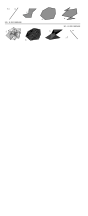
\includegraphics[width=0.85\linewidth]{fig-1.pdf}
        % \textbf{\small Obstacle Structures that can exist in two-dimensional and three-dimensional environments.}\par\medskip
    \end{center}
     \caption{\textbf{Different obstacle structures that can exist in 2D / 3D} \\
     a) 2D point, b) 2D line, c) 2D convex polygon, d) 2D concave polygon, e) 2D convex polygon with same points, f) 3D projection of a 4D mesh, g) 3D mesh, h) 3D polygon, j) 3D point, k) 3D line.}
     \label{one}
\end{figure}

As the dimensionality increases, the perception of obstacles needs to evolve to handle the complexities introduced, like navigating the inside/outside of a 4D tesseract. To cope with these challenges, it becomes essential to simplify the representation of obstacles.

%% buradan yer kazanırsak, simplification için harca



\section{\large \textbf{Potential Function Approach}}

\subsection{Additive Attractive/Repulsive Potentials}
The combination of attractive and repulsive potentials forms the simplest potential function with a straightforward concept: the goal point attracts the robot, while each obstacle repels it. The summation of these effects results in a potential field that guides the robot toward the goal.

\begin{equation*}
    U(q) = U_{att}(q)+ U_{rep}(q)
\end{equation*}

To reach the goal, the robot should traverse from high potential to low potential. This involves defining a change in potential with respect to the dimensions, represented by the gradient. Following the negative gradient, a strategy known as \textit{gradient descent}, leads the robot toward the goal.

The potential function approach offers significant advantages when dealing with high-dimensional problems. The potentials can be easily structured for any number of dimensions, making it a versatile approach. In the subsequent sections, all equations will be presented in their most generic form to accommodate various dimensionalities.
    

\subsubsection{The Attractive Potential}
There are several options available for defining an appropriate attractive potential for the goal. One such option is the conic potential, but it introduces a discontinuity at the point of origin. Alternatively, a quadratic potential can be utilized. This potential grows quadratically as the object approaches, providing a continuously differentiable function. Since it relies solely on distance definition, it can be applied seamlessly across any number of dimensions.
\begin{equation*}
\begin{split}
    U_{att}(q) = \frac{1}{2}\zeta d^2(q,q_{goal}) &= \frac{1}{2} \zeta (q-q_{goal})^\top(q-q_{goal}) \\
    \nabla U_{att}(q) &= \zeta (q-q_{goal})   
\end{split}
\end{equation*}

The norm squared, defined as the transpose multiplication of vectors, is utilized for calculating the potential that will be used to visualize the environment, to better understanding of the system's dynamics.

While the quadratic potential grows significantly for large distances, imposing a heavier computational burden, it becomes necessary to cap it. The transition is then made to the conic potential after reaching a specified distance, denoted as $d^*_{goal}$ distance. This transition forms a new combined field, which can be defined as:
\begin{equation*}
U_{att}(q)=
\begin{cases}
        \frac{1}{2\zeta} d^2(q_{\text{goal}}),  &\text{if } d(q) \leq d^*_{\text{goal}} \\
        d^*_{\text{goal}} \zeta d(q_{\text{goal}}) - \frac{1}{2}\zeta \left(d^*_{\text{goal}}\right)^2,  &\text{if } d(q) > d^*_{\text{goal}}
\end{cases}
\end{equation*}

%ADD THE GRADIENTS HERE ALSO

\subsubsection{The Repulsive Potential}

A repulsive potential used to keep the robot at a distance from obstacles. The intensity of the repulsive force is contingent on the robot's proximity to an obstacle. The closer the robot is to an obstacle, the stronger the repulsive force should be. As a result, the repulsive gradient operates exclusively within a domain near the obstacle. The repulsive potential is commonly defined in terms of the distance to the nearest obstacle, denoted as $D(q)$. The repulsive potential and its gradient is explained in further detail in \cite{choset}.

\begin{equation*}
    U_{\text{rep}}(q) =
    \begin{cases}
        \frac{1}{2}\eta (\frac{1}{D(q)} - \frac{1}{Q^*})^2, & \text{if } D(q) \leq Q^*, \\
        0, & \text{if } D(q) > Q^*.
    \end{cases}
\end{equation*}


\subsubsection{Gradient Descent}
Gradient descent is a commonly used approach for searching solutions to generic optimization problems. The concept is straightforward: starting from the initial configuration, take a small step in the direction opposite to the gradient. This results in a new configuration, and the process iterates until the gradient becomes zero. Formally, a gradient descent algorithm can be defined in Algorithm.~\ref{alg:gradient-descent}.


\begin{algorithm}[b]
\caption{Gradient Descent}
\label{alg:gradient-descent}
\begin{algorithmic}
\Require Gradient $\nabla U(q) $at a point $q$
\Ensure A sequence of points $\{q(0), q(1), ... , q(i)\}$
\algrule
\State $q(0) = q_{start}$
\State $i=0$
\While {$\nabla U(q(i)) \neq 0$} 
    \State $q(i+1) = q(i)+\alpha (i) \nabla U(q(i)) $
    \State $i = i+1$
\EndWhile

\end{algorithmic}
\end{algorithm}

\section{\large \textbf{Implementation}}

In the MATLAB-based simulation environment, the implementation begins by creating a navigable space with uniformly expanded bounds. However, the obstacles are created manually. This introduces challenges, particularly with higher-order obstacles that lack direct physical representation and there is no dimension increase that is interconnected to the robot's changing configuration space. This disconnect poses difficulties in generating meaningful obstacles for algorithm testing. Addressing this challenge is crucial to experiment on high and low dimensional structures where real cases may be applicable to in the future. Obstacles that are consistent are essential to thoroughly test the path planning algorithm hence an approximation is to be made both helping in construction of obstacles and calculations in later steps.

\subsection{Obstacle Approximation}
Beginning with planar environments, the introduction of polygons as obstacles are plausible and logical. Constructing these polygons is relatively straightforward, allowing for flexible placement and sizing that aligns with the requirements of the test environments. The incorporation of polygonal obstacles serves a dual purpose — not only do they facilitate the comparison of different approximations, but they also pose a challenging scenario for evaluating the effectiveness of the potential function approach in terms of path-finding.

In three-dimensional environments, utilizing a mesh as an obstacle is a suitable choice, although constructing these meshes can be a bit intricate. One approach is to generate primitive shapes, or they can be crafted using proprietary software, presenting a challenging yet manageable task.

However, when dealing with dimensions higher than three, there is a lack of tools and established procedures for construction. In such cases, using points on the obstacles becomes a viable alternative. N-dimensional point data known to define an obstacle can be employed to generate a high-dimensional structure that serves as an approximation.

The hyper-sphere approach proves valuable in this context. By utilizing an n-dimensional sphere consistent with the dimension of the environment, the creation of hyper-obstacles becomes relatively simple. Given a collection of points from the obstacle in any dimension, the diameter of the hyper-obstacle can be determined by the distance between the two most distant points, with the center of the hyper-obstacle located at the midpoint of these two extremities.
Obstacle approximation is done once at the beginning, and the approximate map is retained for ongoing analysis during the simulation.

\begin{itemize}
    \item \textbf{Exact Obstacles} : The exact obstacles/polygons is applicable strictly for 2D environments. In such cases, gradients of potentials can be calculated by considering planar distances from the robot's position to the edges of the obstacles. However, in higher dimensions, the edges transition into surfaces and volumes. This complicates distance calculations from the obstacle "surface" to the robot, posing challenges in determining accurate potentials.
    \item \textbf{Approximate Obstacles} : The approximate obstacles involve utilizing only the point data from the actual obstacles. This involves constructing "bounding n-spheres," ensuring that all points lie within the smallest hyper-sphere. This approximation is used in dimensions from three to N. In 2D environments, the approximations simplify to circles for the obstacles, offering a practical comparison setting for the exact and approximate obstacle presentations.
\end{itemize}

\subsection{Solver Selection}
The computation of gradients has been previously explained, and the algorithmic components are straightforward. The path calculation from the gradients involves two approaches. One approach is solving the differential equations more accurately using proprietary solvers, while the other approach involves discrete methods by iteratively taking small steps over the gradients. The implementation incorporates both approaches, allowing for experimentation with various aspects of these different calculation methods. This dual approach enables a comprehensive exploration of the trade-offs and advantages associated with accurate differential equation solvers and iterative discrete methods in the context of path planning. Moreover both of the algorithms are applicable to n-dimensions.

\begin{itemize}
    \item \textbf{ODE45}: A continuous solver that is proven to provide highly accurate and smooth path solutions. It has an adaptive step size, it efficiently computes precise results, making it particularly effective for scenarios where precision is crucial, that is moving through a tight passage. 
    \item \textbf{DISCRETE}: An iterative solver, easily implementable and allowing for the adjustment of step sizes, provides flexibility. However, it may lead to instabilities, including oscillations around minima without achieving convergence. Careful consideration is necessary.
\end{itemize}

The experimentation will include both approaches, comparing their efficacy across dimensions ranging from two to n.

% ending the searcg for ODE and Discrete, different ways and epsilon deifinitions
% \subsection{Visualizations}

% \begin{algorithm}[t]
% \caption{Rotational Plane Sweep Range Sensor}
% \label{alg:rps_sensor}
% \begin{algorithmic}
% \Require $robot\_position(v),$ $arena\_map$
% \Ensure $distance$, $angle$
% \algrule
% \If{robot is out of bounds}
%     \State exit.
% \EndIf
% \State $\mathcal{E} \gets$ number of vertices $\in \ \mathcal{Q}$
% \State $\mathcal{S} \gets$ ordered edges $\in \ \mathcal{Q}$
% \For{\text{$v:$ robot position}} 
%     \If{$v_i$ is visible to $v$}
%         \State Add the edge ($v$,$v_i$) to visibility graph
%     \EndIf
%     \If{$v_i$ is the beginning of an edge, $E$ $\notin$ $\mathcal{S}$}
%         \State insert $E$ into $ \mathcal{S}$
%         \State calculate dist, angle $E$ to $v$
%     \EndIf
%     \If{$v_i$ is the end of and edge in $\mathcal{S}$}
%         \State delete the edge from $\mathcal{S}$
%     \EndIf
% \EndFor

% \end{algorithmic}
% \end{algorithm}

\section{\large \textbf{Experimentation}}
\subsection{2D Experiments}

The simple case serves as a distinct test to compare the discrete and ODE solutions. With uncomplicated obstacles, the path is easily found in both scenarios as the Fig.~(\ref{simple}) laying out. The step size for the DISCRETE option was set at 0.1, leading to a jittery motion along the path. The resulting path also exhibits a similarity to the Greedy Bug and Bug-2 algorithms, wherein the robot follows the boundary until it can directly sense the direction of the goal. Concave obstacles were deliberately chosen to minimize the risk of encountering local minima. The upcoming test will focus specifically on scenarios designed to further eliminate the possibility of local minima.

The variables $\zeta$ and $\eta$ play a crucial role in modifying both attractive and repulsive potential fields, and their values are determined experimentally. Ensuring that adjustments to one variable do not adversely impact the other is a challenge, especially in cases where close or complex-shaped obstacles are involved. While calibration is straightforward in many instances, obstacles with intricate shapes or close proximity often require numerous tweaks to strike the right balance.

\begin{figure}[t]
    \begin{center}    
        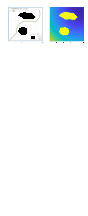
\includegraphics[width=1\linewidth]{simple.pdf}
    \end{center}
     \caption{Path from "ODE45" and "DISCRETE" approaches on the left and potential function shown on the right.}
     \label{simple}
\end{figure}

\begin{figure}[t]
    \vspace{-1em}
    \begin{center}    
        \includegraphics[width=0.8\linewidth]{simple-pot.png}
    \end{center}
     \caption{3D visualization of the potential function for the simple case.}
     \label{simple-pot}
\end{figure}

In the second test, the starting point and goal remain unchanged, but the obstacle approximation is modified. The 2-sphere approximation now encapsulates the entire obstacles, including the available paths around them. However, a notable issue arises as the new obstacles are positioned closer to each other, creating a local minima point in between. Consequently, the algorithm struggles to find a viable path.

This example highlights a couple of problems with the approximation. Notably, thin and long obstacles are approximated to circles, consuming a significant portion of the free space and affecting the algorithm's ability to navigate through complex configurations.

\begin{figure}
    \vspace{-1em}
    \begin{center}    
        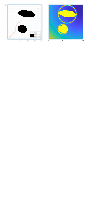
\includegraphics[width=1\linewidth]{simple-2.pdf}
    \end{center}
     \caption{Simple case with obstacles are approximated, the solution cannot be found.}
     \label{simple-2}
\end{figure}

\begin{figure}
    \vspace{-1em}
    \begin{center}    
        \includegraphics[width=0.8\linewidth]{simple-approx-pot.png}
    \end{center}
     \caption{Potential field for the simple case with obstacle approximation.}
     \label{simple-approx-2}
\end{figure}

In the upcoming test, specific convex polygons are introduced, designed to act like cups that can trap the robot along its path to the goal. If these obstacles are strategically placed in the available path, it becomes challenging for the robot to escape from the resulting local minima. One potential solution could involve increasing the repulsive potential. However, this approach poses a dilemma, as increasing repulsion may cause the obstacle to resemble a point-like structure, necessitating a corresponding increase in the attractive potential. Striking the right balance between these potentials becomes crucial for successful path planning through environments with strategically placed convex obstacles.

The approximate hyper-sphere approach proves efficacy in transforming convex obstacles into concave hyperdimensional entities. This methodology contributes to eliminating local minima, thereby generating a more viable solution in complex environments.

\begin{figure}
    \vspace{-1em}
    \begin{center}    
        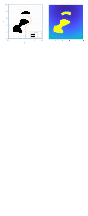
\includegraphics[width=0.8\linewidth]{simple-3.pdf}
    \end{center}
     \caption{Cup case with exact obstacles, the path cannot be found.}
     \label{three}
\end{figure}

\begin{figure}
    \vspace{-1em}
    \begin{center}    
        \includegraphics[width=0.8\linewidth]{cup-pot.png}
    \end{center}
     \caption{Potential field representation in 3D for the Cup case.}
     \label{three}
\end{figure}



\begin{figure}
    \vspace{-1em}
    \begin{center}    
        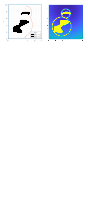
\includegraphics[width=0.8\linewidth]{simple-4.pdf}
    \end{center}
     \caption{Cup case with approximated obstacles, the solution is closer to the goal.}
     \label{three}
\end{figure}

\begin{figure}
    \vspace{-1em}
    \begin{center}    
        \includegraphics[width=0.8\linewidth]{cup-pot-approx.png}
    \end{center}
     \caption{The potential field plot for the approximated cup case.}
     \label{three}
\end{figure}


\begin{figure}[b]
    \vspace{-1em}
    \begin{center}    
        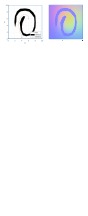
\includegraphics[width=0.8\linewidth]{swirl-1.pdf}
    \end{center}
     \caption{Hard case as a single obstacle twirls.}
     \label{three}
\end{figure}

% \begin{figure}[b]
%     \vspace{-1em}
%     \begin{center}    
%         \includegraphics[width=0.8\linewidth]{swirl-pot-3.png}
%     \end{center}
%      \caption{Potential for the Hard case, where the color in RGB shows the gradient of the surface.}
%      \label{three}
% \end{figure}

% \begin{figure*}[t]
%     \centering
%     \begin{subfigure}[t]{0.5\textwidth}
%         \centering
%         \includegraphics[height=2in]{swirl-pot-2.png}
%         \caption{Lorem ipsum}
%     \end{subfigure}%
%     ~ 
%     \begin{subfigure}[t]{0.5\textwidth}
%         \centering
%         \includegraphics[height=2in]{swirl-pot.png}
%         \caption{Lorem ipsum, lorem ipsum,Lorem ipsum, lorem ipsum,Lorem ipsum}
%     \end{subfigure}
%     \caption{Caption place holder}
% \end{figure*}


\begin{figure}
  \centering
  \begin{subfigure}{.5\columnwidth}
    \centering
    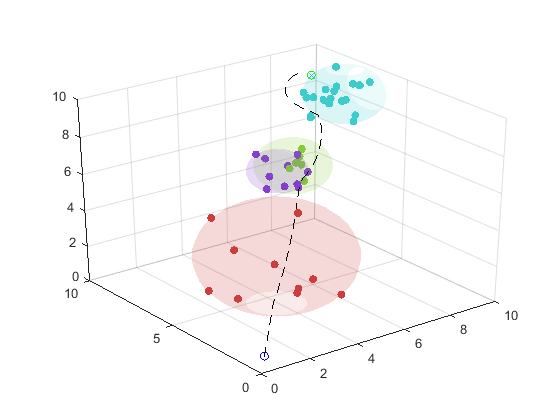
\includegraphics[width=\linewidth]{three-6.pdf}
    \caption{Three dimensional solution with obstacles are approximated and the path is found.}
  \end{subfigure}%
  \hfill
  \begin{subfigure}{.5\columnwidth}
    \centering
    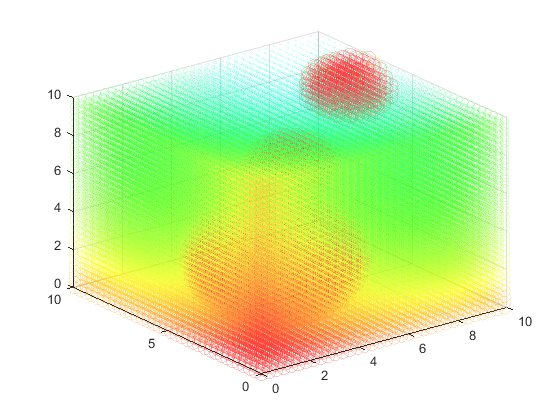
\includegraphics[width=\linewidth]{three-pot-6.pdf}
    \caption{The related potential function that is a volumetric scalar visualization.}
  \end{subfigure}%
\end{figure}






% \begin{figure}[b]
%     \vspace{-1em}
%     \begin{center}    
%         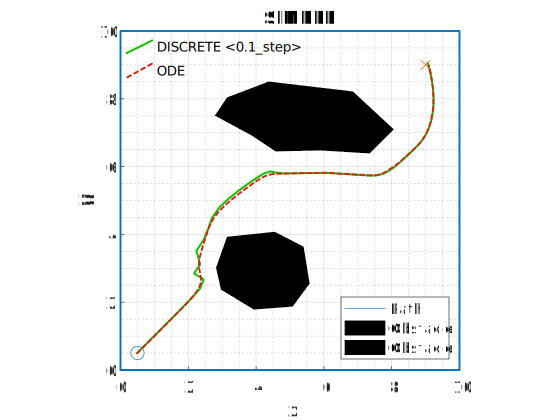
\includegraphics[width=1\linewidth]{fig-3.pdf}
%     \end{center}
%      \caption{}
%      \label{three}
% \end{figure}

\begin{figure*}
  \begin{subfigure}{0.33\textwidth}
    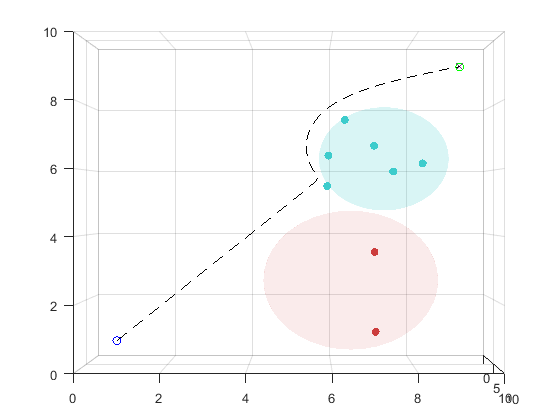
\includegraphics[width=\linewidth]{three-3.pdf}
    \caption{}
    \label{fig:figure1}
  \end{subfigure}%
  \hfill
  \begin{subfigure}{0.33\textwidth}
    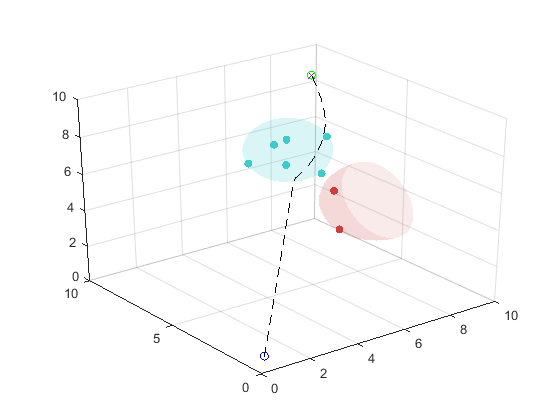
\includegraphics[width=\linewidth]{three-1.pdf}
    \caption{}
    \label{fig:figure2}
  \end{subfigure}%
  \hfill
  \begin{subfigure}{0.33\textwidth}
    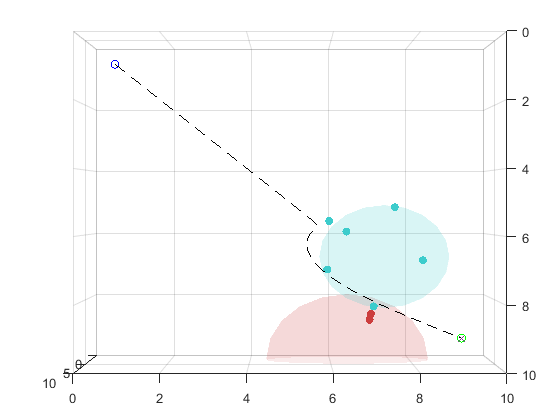
\includegraphics[width=\linewidth]{three-2.pdf}
    \caption{}
    \label{fig:figure3}
  \end{subfigure}
  \caption{Three dimensional path finding using potential functions, path is found.}
\end{figure*}
\subsection{3D Experiments}

Displaying three-dimensional examples poses more challenges, but the path planning algorithm remains consistent. In these scenarios, the potential visualizations are volumetric, with the color intensity indicating the degree of repulsion; deeper shades of red signify higher repulsive forces, as evident in the figures.


\begin{figure*}
    \vspace{-1em}
    \begin{center}    
        \includegraphics[width=1\linewidth]{fourth.pdf}
    \end{center}
     \caption{Three dimensional projections of the fourth dimensional environments, the path is found consisting of a four dimensional vector. The figures above are orthogonal to each other.}
     \label{three}
\end{figure*}

\subsection{4D Experiments}
Extending the solution to four dimensions is as straightforward as adding one more dimension, although visualizations become more challenging. The figure below illustrates projections of the fourth-dimensional environment and the found path onto four distinct three-dimensional plots. Despite the complexity, the path is successfully found, and obstacles are approximated using high-dimensional spheres.
% \subsection{Observations}


% \section{\large \textbf{Conclusion}}

% \section{\large \textbf{Conclusion}}

\bibliographystyle{bib/IEEEtaes}

\bibliography{bib/refs}\ %IEEEabrv instead of IEEEfull

\end{document}
